\subchapter{Configuring pin muxing}
{Objective: learn how to declare and use a muxing state.}

\section{Goals}

As part of the previous lab, we enabled an I2C controller and described
a device plugged on the bus. In this lab we will cover how to ensure a
proper communication between the two and be able to declare and use
pinctrl settings.

\section{Setup}

Continue using the \code{bbb-custom} branch in the
\code{~/linux-kernel-labs/src/linux} directory.

\section{Probing the different busses}

Now, let's use \code{i2cdetect}'s capability to probe a bus for
devices. The I2C bus has no real discovery capability, but yet, the tool
exploits a feature of the specification: when the master talks to a
device, it starts by sending the target address on the bus and expects
it to be acked by the relevant device. Iterating through all the
possible addresses without sending anything after the address byte,
looking for the presence of an Ack is what uses the tool to probe the
devices. That is also why we get a warning when using it.

Let's start by probing the bus associated to \code{i2c-0}:

\begin{bashinput}
# i2cdetect -r 0
i2cdetect: WARNING! This program can confuse your I2C bus
Continue? [y/N] y
     0  1  2  3  4  5  6  7  8  9  a  b  c  d  e  f
00:          -- -- -- -- -- -- -- -- -- -- -- -- --
10: -- -- -- -- -- -- -- -- -- -- -- -- -- -- -- --
20: -- -- -- -- UU -- -- -- -- -- -- -- -- -- -- --
30: -- -- -- -- 34 -- -- -- -- -- -- -- -- -- -- --
40: -- -- -- -- -- -- -- -- -- -- -- -- -- -- -- --
50: 50 -- -- -- -- -- -- -- -- -- -- -- -- -- -- --
60: -- -- -- -- -- -- -- -- -- -- -- -- -- -- -- --
70: -- -- -- -- -- -- -- --
\end{bashinput}

We can see three devices on this internal bus:
\begin{itemize}
\item One at address \code{0x24}, indicated by \code{UU},
      which means that there is a kernel driver actively
      driving this device.
\item Two other devices at addresses \code{0x34} and \code{0x50}.
      We just know that they are currently not bound to a kernel driver.
\end{itemize}

Now try to probe I2C1 with \code{i2cdetect -r 1}.

You will see that the command will fail to connect to
the bus. That's because the corresponding signals are
not exposed yet to the outside connectors through pin muxing.

\section{Find pin muxing configuration information for i2c1}

As you found in the previous lab, we now managed to have our nunchuk
device enumerated on the \code{i2c1} bus.

However, to access the bus data and clock signals, we need to configure
the pin muxing of the SoC.

If you go back to the BeagleBone Black System Reference Manual, in the
{\em Connector P9} section, you can see that the pins \code{17} and
\code{18} that we are using correspond to pins \code{A16} and \code{B16}
of the AM335 SoC. You can also see that such pins need to be configured
as \code{MODE2} to get the functionality that we need (\code{I2C1_SCL}
and \code{I2C1_SDA}).

The second step is to open the CPU datasheet (\code{am3359.pdf}), and
look for pin assignment information ({\em Pin Assignments} section).
You will find that the processor is available through two types of
packages: \code{ZCE} and \code{ZCZ}. If you have an original
BeagleBoneBlack board, you can have a very close look at the CPU
(with your glasses on!) and you will see that the CPU has \code{ZCZ} written
on its lower right corner. On BeagleBoneBlack Wireless with the
Octavo System In Package, you can no longer find such information.
Anyway, the \code{ZCZ} package information applies to both types of
boards.

So, in the {\em ZCZ Package Pin Maps (Top View)} section\footnote{Caution: you
won't be able to search the PDF file for this section name, for obscure
reasons. At the time of this writing, this section is numbered 4.1.2.}, you can find
hyperlinks to the descriptions of the \code{A16} and \code{B16} pins.
That's where you can find reference pin muxing information for these
pins.  You can find that the pin name for \code{A16} is \code{SPI0_CS0}
and that the pin name for \code{B16} is \code{SPI0_D1}.
You can also get confirmation that to obtain the (\code{I2C1_SCL} and
\code{I2C1_SDA}) signals, you need to configure muxing mode number 2.
You can also see that both pins support pull-up and pull-down
modes\footnote{See \url{https://en.wikipedia.org/wiki/Pull-up_resistor}}
(see the \code{PULLUP /DOWN TYPE} column).

The next thing to do is to open the big TRM document and look for the
address of the registers that control pin muxing. First, look for
{\em L4\_WKUP Peripheral Memory Map} with your PDF reader search
utility. You will find a table containing a
\code{Control Module Registers} entry with its address:
\code{0x44E1_0000}.

Last but not least, look for the \code{SPI0_CS0} and \code{SPI0_D1}
pin names, and you will find the offsets for the registers controlling
muxing for these pins in the {\em CONTROL\_MODULE REGISTERS} table:
respectively \code{0x95c} and \code{0x958}.

We now know which registers we can write to to enable \code{i2c1}
signals.

\section{Multiplexing the I2C controller outputs correctly}

Now that we know the register offsets, let's try to understand
how they are used in existing code. For example, open the
the Device Tree for the AM335x EVM board
(\kfile{arch/arm/boot/dts/ti/omap/am335x-evm.dts}), which is using
\code{i2c1} too. Look for \code{i2c1_pins}, and you will see how
offsets are declared and what values they are given:

{\small
\begin{verbatim}
i2c1_pins: i2c1-pins {
        pinctrl-single,pins = <
                /* spi0_d1.i2c1_sda */
                AM33XX_PADCONF(AM335X_PIN_SPI0_D1, PIN_INPUT_PULLUP, MUX_MODE2)
                /* spi0_cs0.i2c1_scl */
                AM33XX_PADCONF(AM335X_PIN_SPI0_CS0, PIN_INPUT_PULLUP, MUX_MODE2)
        >;
};
\end{verbatim}
}

Here are details about the values:

\begin{itemize}
\item \ksym{AM335X_PIN_SPI0_D1} and \ksym{AM335X_PIN_SPI0_CS0} offsets
      in the Pin Controller registers to control muxing on the
      corresponding package pins.
\item \ksym{MUX_MODE2} corresponds to muxing mode 2, as explained in the
      datasheet.
\item \ksym{PIN_INPUT_PULLUP} puts the pin in pull-up mode (remember
      that our pins support both pull-up and pull-down). By design, an
      I2C line is never actively driven high, devices either pull the
      line low or let it floating. As we plug our device directly on the
      bus without more analog electronics, we need to enable the
      internal pull-up.
\end{itemize}

Now that pin muxing settings have been explained, edit your board
DTS file to add the same definitions to enable pin muxing for \code{i2c1}.
Don't forget that you don't have to repeat definitions that are
already present in the \code{.dtsi} files. Just add new declarations, or
settings that override common definitions.

Rebuild and update your DTB, and eventually reboot the board. You should
now be able to probe your bus:

\begin{bashinput}
# i2cdetect -r 1
i2cdetect: WARNING! This program can confuse your I2C bus
Continue? [y/N] y
     0  1  2  3  4  5  6  7  8  9  a  b  c  d  e  f
00:          -- -- -- -- -- -- -- -- -- -- -- -- --
10: -- -- -- -- -- -- -- -- -- -- -- -- -- -- -- --
20: -- -- -- -- -- -- -- -- -- -- -- -- -- -- -- --
30: -- -- -- -- -- -- -- -- -- -- -- -- -- -- -- --
40: -- -- -- -- -- -- -- -- -- -- -- -- -- -- -- --
50: -- -- -- -- -- -- -- -- -- -- -- -- -- -- -- --
60: -- -- -- -- -- -- -- -- -- -- -- -- -- -- -- --
70: -- -- -- -- -- -- -- --
\end{bashinput}

No devices are detected, because we did not wire the nunchuk yet.

\subsection{Wiring the I2C device}

Let's connect the Nunchuk provided by your instructor
to the I2C1 bus on the board, using breadboard wires:

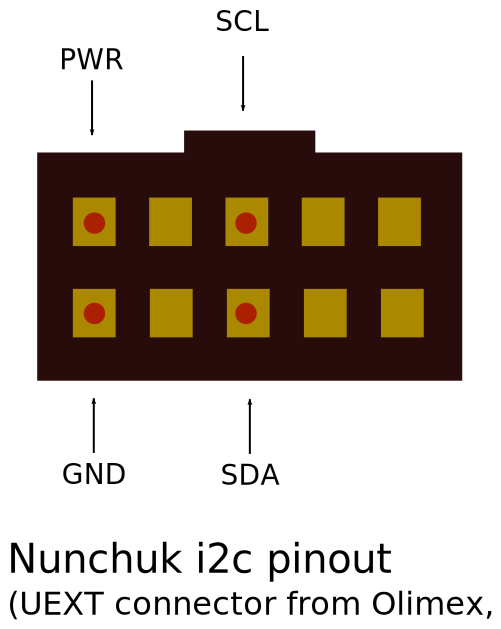
\includegraphics[width=0.3\textwidth]{common/nunchuk-pinout.pdf}
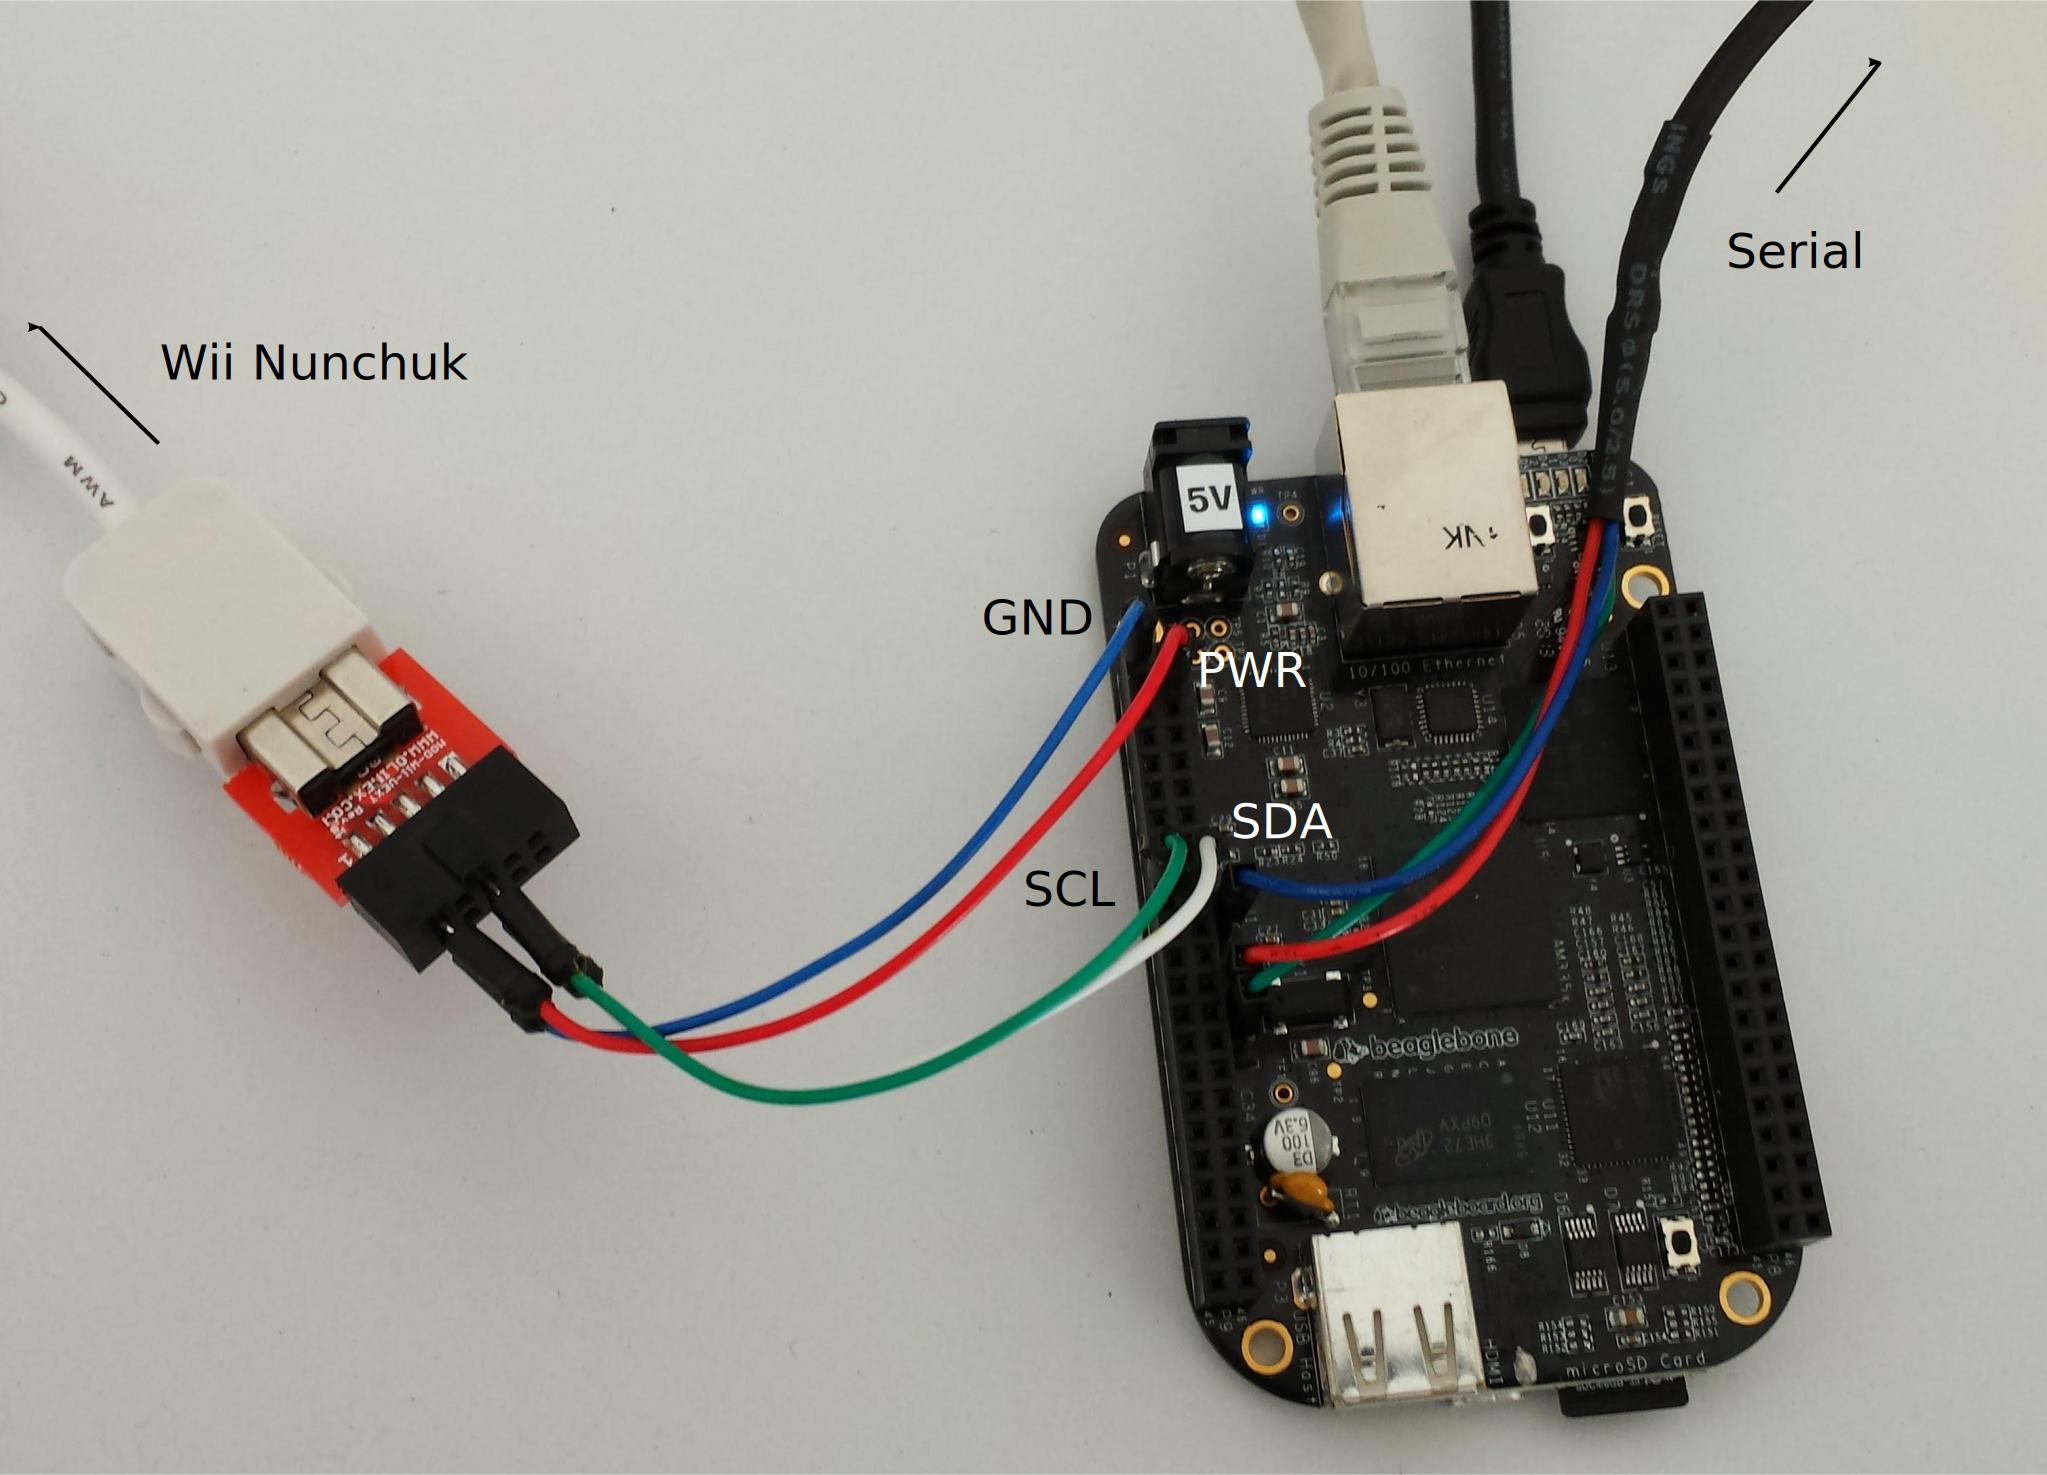
\includegraphics[width=0.7\textwidth]{common/bbb-connect-nunchuk.pdf}

\begin{itemize}
\item Connect the Nunchuk PWR pin to pin 4 (3V3) of connector P9
\item Connect the Nunchuk GND pin to pin 1 (GND) of connector P9
\item Connect the Nunchuk SCL pin to pin 17 of connector P9
\item Connect the Nunchuk SDA pin to pin 18 of connector P9
\end{itemize}

If you didn't do any mistake, your new device should be detected at
address \code{0x52}:

\begin{bashinput}
# i2cdetect -r 1
i2cdetect: WARNING! This program can confuse your I2C bus
Continue? [y/N] y
     0  1  2  3  4  5  6  7  8  9  a  b  c  d  e  f
00:          -- -- -- -- -- -- -- -- -- -- -- -- --
10: -- -- -- -- -- -- -- -- -- -- -- -- -- -- -- --
20: -- -- -- -- -- -- -- -- -- -- -- -- -- -- -- --
30: -- -- -- -- -- -- -- -- -- -- -- -- -- -- -- --
40: -- -- -- -- -- -- -- -- -- -- -- -- -- -- -- --
50: -- -- 52 -- -- -- -- -- -- -- -- -- -- -- -- --
60: -- -- -- -- -- -- -- -- -- -- -- -- -- -- -- --
70: -- -- -- -- -- -- -- --
\end{bashinput}

We will later compile an out-of-tree kernel module to support this device.
